\section{Pile ou face avec \mb}

%   logo mb dans la table des matières
\logo{mb}

% style de page micro:bit
\pagestyle{mb}

\subsection{Description}

\subsubsection{Objectif}

\begin{formule}
Le but de ce projet est de simuler une expérience aléatoire de lancer de pièce avec une carte \mb.

À partir d’une situation simple, idéale pour une prise en main de l’interface de programmation, il s’agit par la suite d’améliorer le programme pas à pas. L’objectif est d’obtenir un programme utilisable dans le cadre d’un cours sur les statistiques et les probabilités.
\end{formule}

\subsubsection{Intérêt}
Bien évidemment, travailler avec une carte \mb n'exclut pas de réaliser des expériences aléatoires réelles (pièces, dés, etc.). Cependant, il est très intéressant pour l'enseignant d'utiliser des \mb dans cette partie du programme.
\begin{description}
    \item [Simplicité de la situation.] La situation est très simple à expliquer et les élèves comprennent le but à atteindre. L'absence de difficulté mathématique rend cette situation particulièrement simple à mettre en œuvre.
    \item [Motivation des élèves.] L'envie de programmer un objet connecté est grande pour les élèves. Cette façon de programmer, \emph{utile, concrète et appliquée}, leur correspond parfaitement.
    \item [De nombreuses solutions/améliorations possibles.] Comme pour bien des projets, il y a plusieurs façons d'arriver à la solution. Par ailleurs, les élèves peuvent apporter ou proposer de nombreuses améliorations. La programmation par bloc, exempte de difficulté syntaxique, est particulièrement adaptée à la créativité.
    \item [Travail mathématique sur la modélisation.] Cette compétence n'est pas facile à mettre en œuvre. Ici, l'absence de difficultés mathématiques rend ce travail beaucoup plus accessible à tous.
\end{description}


\subsubsection{Matériel}
\begin{itemize}
    \item 1 $\times$ \matosMb \emph{(facultatif car le simulateur peut suffire)}
    \item 1 $\times$ accès internet : IDE programmation par bloc \url{http://makecode.microbit.org/}
\end{itemize}



%
% activité de niveau 1
%
\newpage
\subsection{Niveau simple}
\subsubsection{Activité élève}

% commande perso \CARTOUCHE
%   5 paramètres : 
%       * durée
%       * public
%       * travail en maths
%       * travail en sciences
%       * travail en algo
\cartouche{0,5 h}{2de}{expérience aléatoire}{}{affichage ; boucle ; événement.}



\begin{wrapfigure}[4]{r}{3.5cm}
    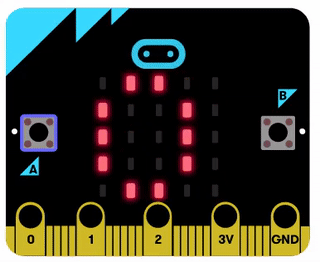
\includegraphics[width=\linewidth]{res/mbPileFaceN1.png}
\end{wrapfigure}
\begin{eleve}
\texttt{\scshape{Mission : }
Utilise \mb~pour jouer à \emph{Pile ou Face} !}

En t'aidant des blocs ci-dessous, programme \mb~pour : 
\begin{enumerate}
    \item afficher une courte animation ;
    \item afficher \emph{de façon aléatoire} \texttt{0} ou \texttt{1}.
\end{enumerate}

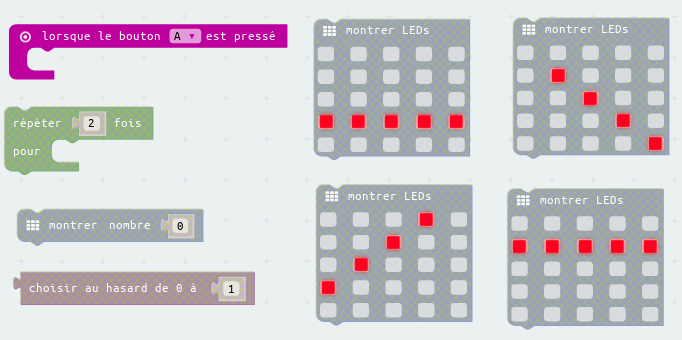
\includegraphics[width=\textwidth]{res/mbPileFaceN1blocs}

\end{eleve}


\newpage
\subsubsection{Notes pour l'enseignant}

Ce premier niveau permet de se familiariser avec l’interface tout en produisant un premier programme fonctionnel et utile.

\begin{minipage}[t]{0.5\linewidth}
    \begin{methode}~\\
    Pour résoudre ce problème, il suffit de programmer les instructions de la façon suivante :
    
    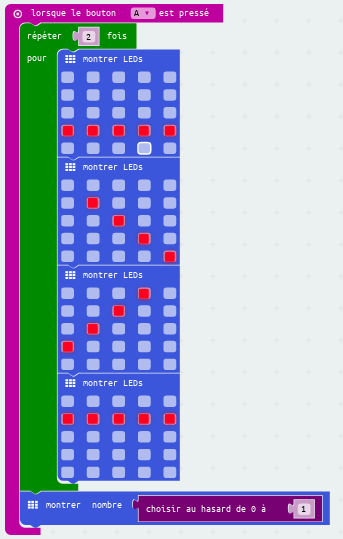
\includegraphics[width=\linewidth]{mbPilefaceN1proposition}
    \end{methode}
\end{minipage}
\hfill
\begin{minipage}[t]{0.5\linewidth}
    \begin{remarque}~\\
    Plus d'informations sur la page de l'activité :\\ \url{https://microbit.readthedocs.io/fr/latest/decouverte/pileface-bloc1.html}
    \end{remarque}
\end{minipage}









%
% activité de niveau 2
%
\newpage
\subsection{Niveau intermédiaire}
\subsubsection{Activité élève}

% commande perso \CARTOUCHE
%   5 paramètres : 
%       * durée
%       * public
%       * travail en maths
%       * travail en sciences
%       * travail en algo
\cartouche{0,5 h}{2de}{expérience aléatoire}{}{affichage ; boucle ; événement ; condition ; fonction.}


\begin{wrapfigure}[4]{r}{3.5cm}
    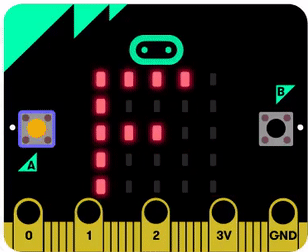
\includegraphics[width=\linewidth]{res/mbPileFaceN2.png}
\end{wrapfigure}
\begin{eleve}
Maintenant, {\Large{améliore}} le programme de ton \mb.

Voici deux idées :
\begin{itemize}
    \item au lieu d'afficher \texttt{0} ou \texttt{1}, affiche plutôt \texttt{P} ou \texttt{F} ;
    \item utilise une fonction pour gérer ton animation.
\end{itemize}
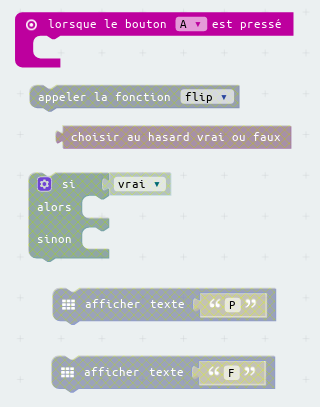
\includegraphics[width=0.5\textwidth]{res/mbPilefaceN2blocs.png}
\end{eleve}


\newpage
\subsubsection{Notes pour l'enseignant}

Ce deuxième niveau est l'occasion d'introduire les notions de fonctions et les branchements conditionnels.

\begin{methode}
Voici une proposition qui fonctionne :

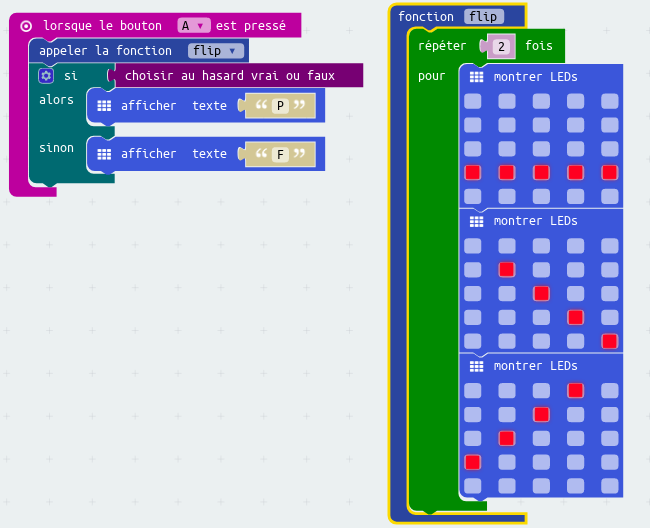
\includegraphics[width=\linewidth]{res/mbPilefaceN2proposition.png}
\end{methode}

\begin{remarque}
Plus d'informations sur la page de l'activité :\\ \url{https://microbit.readthedocs.io/fr/latest/decouverte/pileface-bloc2.html}
\end{remarque}





%
% activité de niveau 3
%
\newpage
\subsection{Niveau expert}
\subsubsection{Activité élève}

% commande perso \CARTOUCHE
%   5 paramètres : 
%       * durée
%       * public
%       * travail en maths
%       * travail en sciences
%       * travail en algo
\cartouche{0,5 h}{2de}{expérience aléatoire}{}{affichage ; boucle ; événement ; condition ; fonction ; variable (incément) ; texte (concaténation).}


\begin{wrapfigure}[4]{r}{2.5cm}
    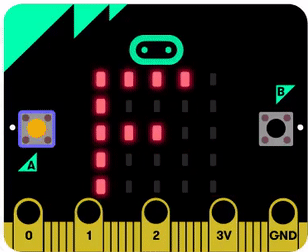
\includegraphics[width=\linewidth]{res/mbPileFaceN2.png}
\end{wrapfigure}
\begin{eleve}
Est ce que \mb peut afficher les tirages obtenus ?

Pour finir, nous souhaitons ajouter une fonctionnalité supplémentaire à \mb. Il faut maintenant arriver à afficher l'effectif total pour les \texttt{Piles} et pour les \texttt{Faces}.

Regarde ci-dessous les instructions que tu pourrais ajouter.

\centerline{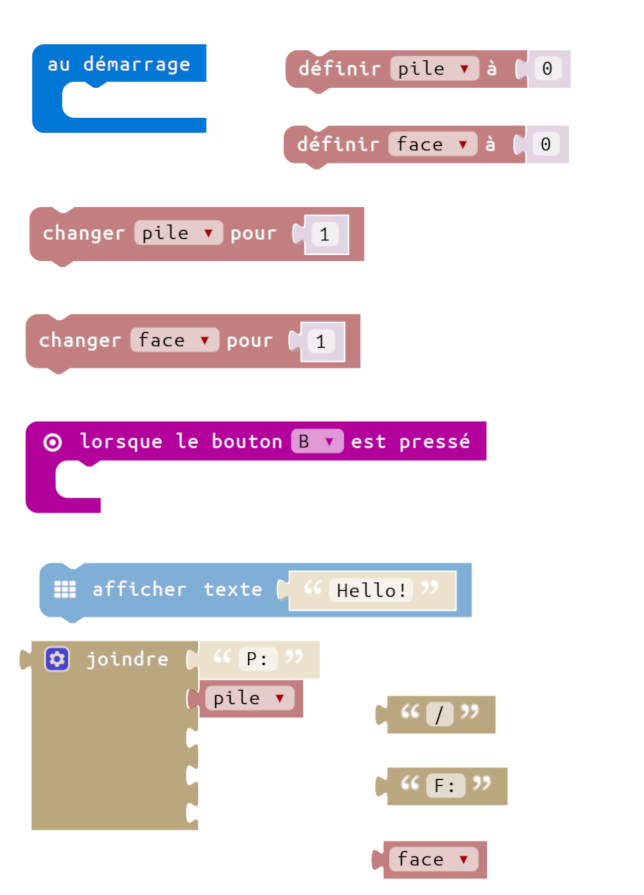
\includegraphics[width=0.4\textwidth]{mbPilefaceN3blocs.png}}
\end{eleve}



\newpage
\subsubsection{Notes pour l'enseignant}

Dans ce troisième niveau, nous souhaitons compter les issues obtenues et afficher les totaux. Il faut introduire la notion de variable informatique.

\begin{methode}
Le résultat escompté est le suivant :\\
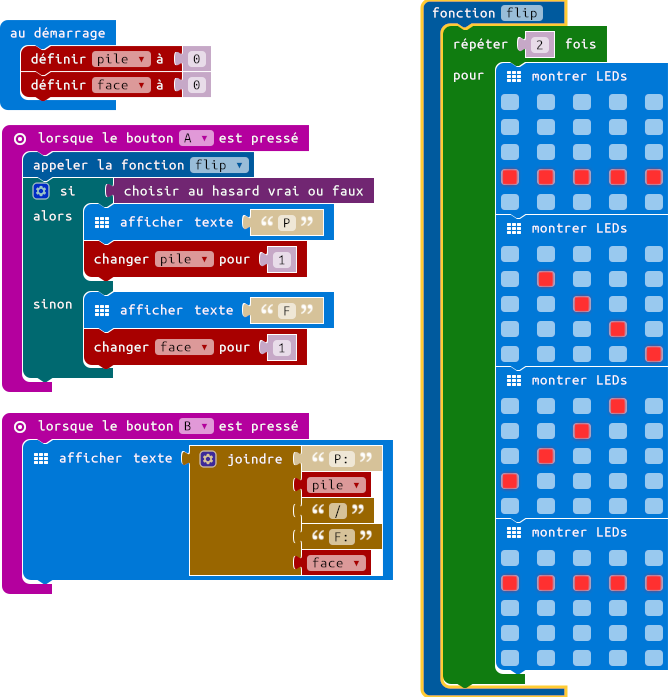
\includegraphics[width=\linewidth]{res/mbPilefaceN3proposition.png}
\end{methode}

\begin{remarque}
Plus d'informations sur la page de l'activité :\\ \url{https://microbit.readthedocs.io/fr/latest/decouverte/pileface-bloc3.html}
\end{remarque}


